% !TeX root = ./main.tex

%\begin{algorithm}[t!]
%	
%	\KwData{Solution genotype $g$, total num. of VMs $N^T$, num. VMs per server $N^V$, set of services $S$}
%	\KwResult{Balanced solution $g$ modified in place}
%
%	$F \gets \emptyset$ \tcp{Set of free VMs}
%
%	$P \gets \emptyset$ \tcp{Set of used VMs}
%
%	\For{$s \in S$} {
%		$N^I_s \gets 0$ \tcp{Number of instances of service $s$}
%	}
%	
%	\tcc{\textbf{1. Find used/free VMs}}
%	\For{$i \gets 0$ \KwTo $N^T$} {
%		\eIf{$g_i = \texttt{None}$}{
%			\tcp{Record location of free VMs}
%			$F \gets F \cup i$
%		}{
%			\tcp{Record location of service instances}
%			$s \gets g_i$
%
%			$P \gets P \cup (i, s)$
%
%			$N^I_s \gets N^I_s + 1$
%		}
%	}
%	\tcc{\textbf{2. Find size of solution after mapping}}
%
%	$N^U \gets 0$ \tcp{Total num. VMs used after mapping}
%
%	\For{$s \in S$}{
%		$L_s \gets 0$ \tcp{Num. VMs used by the service}
%
%		\eIf{$s \in \mathcal{A}$}{
%			$L_s \gets \left\lceil \abs{s} / N^V \right\rceil \cdot N^V$
%		}{
%			$L_s \gets |S_i|$
%		}
%		$N^U \gets N^U + L_s \cdot N_s^I$
%	}
%	\tcc{\textbf{3. Assign missing services to free spaces}}
%	$M \gets \emptyset$ \tcp{Set of missing services}
%	\For{$s \in S$}{
%		\If{$N^I_s = 0$}{
%			$M \gets M \cup s$
%		}
%	}
%
%	\While{$\abs{M} > 0 $ and $ \abs{F} > 0$}{
%		$i \gets \text{\textbf{pop} first free VM from} \; F$
%
%		$s \gets \text{\textbf{pop} first missing service from} \; M$
%
%		$g_i \gets s$ \tcp{Assign service to VM}
%
%		$N^U \gets N^U + L_s$
%	}
%
%	\tcc{\textbf{4. Swap service instances until feasible}}
%
%	\textbf{Sort} service instances in $P$ by their contribution (\pref{eq:contribution}) in ascending order
%
%	\While{$N^U > N^T$ or $\abs{M} > 0$} {
%		$(i, s) \gets $ \textbf{pop} first service instance in $P$
%
%		$g_i \gets \texttt{None}$ \tcp{Free VM}
%
%		$N^U \gets N^U - L_s$
%
%		\If{$\abs{M} > 0$}{
%			$s \gets \textbf{pop } \text{first missing service from } M$ 
%
%			$g_i \gets s$
%
%			$N^U \gets N^U + L_s$
%		}
%	}
%	\caption{Balances the number of instances of each service to ensure feasibility.}
%	\label{alg:balance}
%\end{algorithm}

\section{Proposed Evolutionary Optimization Framework for VNFPPs}
\label{sec:optimisation}

In this section, we propose a tailored evolutionary optimization framework to solve the three-objective VNFPP defined in~\pref{sec:problem_formulation}. There are two tailored features: one is a genotype-phenotype solution representation, detailed in~\pref{sec:representation}, that guarantees feasible solutions for the underlying VNFPP; the other is a tailored initialization operator, detailed in~\pref{sec:operators}, built upon the solution representation to produce a good initial population. Note that these tailored features can be readily incorporated into any existing EMO algorithm as shown in~\pref{sec:incorporation}. Although these operators are specifically designed for the Fat Tree network topology~\cite{AlFaresLV08} (see~\pref{fig:topology}) given its wide adoption in industry~\cite{LebiednikMT16}, we argue that our model and problem formulation are generally useful for any network topology.

\subsection{Genotype-Phenotype Solution Representation}
\label{sec:representation}
%A poor solution representation largely leads to an ineffective search process. 
\textcolor{red}{One of the key challenges when designing and/or applying EAs to real-world optimization problems is how to encode the problem into a solution in EA. In this paper, we propose a genotype-phenotype solution representation for our VNFPP. As shown in \pref{fig:gp_mapping}, the genotype is a string of characters where each character can be either a service $s\in S$ or a sentinel \texttt{NONE}, i.e., the corresponding VM is not in use (illustrated in the figure with an empty character). The phenotype is a set of paths and the corresponding path probabilities required for the VNFPP. The mapping between them defines how to transform the genotype into the corresponding phenotype. Due to the existence of complex constraints defined in~\pref{sec:problem_formulation}, a simple mapping does not always lead to a feasible solution. The main crux of our genotype-phenotype solution representation is the use of problem-specific heuristics at the mapping stage that avoid generating infeasible solutions. It consists of three steps: \texttt{balance}, \texttt{placement} and \texttt{routing}.}

\begin{figure*}[t!]
	\begin{subfigure}[T]{.3\linewidth}
		\centering
		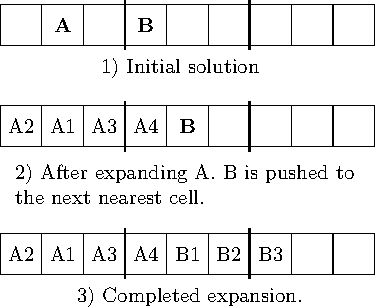
\includegraphics[width=\columnwidth]{figures/simple_expansion-crop}
		\caption{Simple expansion.}
		\label{fig:1a}
	\end{subfigure}\hfil
	\begin{subfigure}[T]{.3\linewidth}
		\centering
		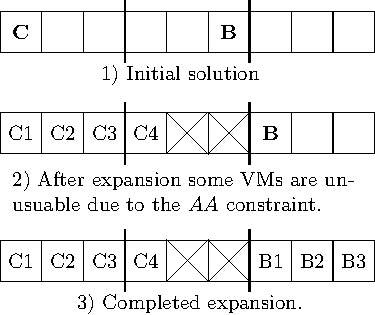
\includegraphics[width=\columnwidth]{figures/aa_expansion-crop}
		\caption{Anti-affinity expansion.}
		\label{fig:1b}
	\end{subfigure}\hfil
	\begin{subfigure}[T]{.3\linewidth}
		\centering
		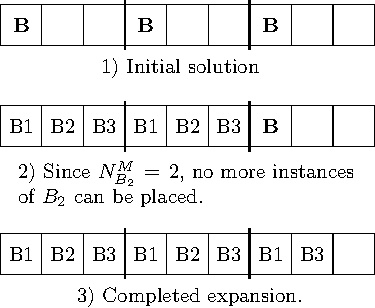
\includegraphics[width=\columnwidth]{figures/limited_expansion-crop}
		\caption{Max instances expansion}
		\label{fig:1c}
	\end{subfigure}
	\vspace{2em}
	\caption{This figures shows three examples of the placement step of the genotype-phenotype mapping. There are three services here: service $\mathbf{A} = \{ A_1, A_2, A_3, A_4\}$ , service $\mathbf{B} = \{B_1, B_2, B_3\}$ which has a max instances constraint $N_{B_2}^M = 2$ and service $\mathbf{C} = \{C_1, C_2, C_3, C_4\}$. In addition, $\mathcal{A} = \{C\}$ such that service $\mathbf{C}$ cannot share a server with any other service. Tall lines indicate server boundaries.}
	\label{fig:placement}
\end{figure*}


\subsubsection{Balance}

The \texttt{balance} step adds and/or removes service instances to guarantee the feasibility after the genotype-phenotype mapping. This is implemented by ensuring that the genotype has at least one instance of each service and the total number of VMs being used does not exceed the available number in the data center. The pseudo-code is given in Algorithm 3 in Appendix C. It first identifies the location of all unused VMs along with the location and number of each service instance (lines 6 to 14). Using this information, the algorithm can calculate the number of VMs the solution will require after the mapping (lines 16 to 23) and identify missing services that have no service instances (lines 24 to 28). The algorithm then places a service instance for any missing services on a free VM if possible (lines 29 to 33). Finally, if there is insufficient space to place a missing service instance or the expanded length of the solution would exceed the total capacity, the algorithm removes the service instance with the lowest contribution and, if necessary, replaces it with a service instance for a missing one (lines 35 to 43). In particular, the contribution of an instance is evaluated as the change in the service instance utilization if it were removed:
\begin{equation}
	C^s_i = \frac{\lambda_{s}}{\mu_{s_1} \cdot (i - 1)} - \frac{\lambda_{s}}{\mu_{s_1} \cdot i},
	\label{eq:contribution}
\end{equation}
\noindent where $C^s_i$ is the contribution of the $i$th instance of $s$ and $\mu_{s_1}$ is its service rate of the first VNF. As the arrival rate is distributed over each VNF, a service with several instances will have some instances with a low contribution. On the other hand, if a service has only one instance, it will have an infinite contribution. This minimizes the impact on the service quality when removing solutions. 

\subsubsection{Placement}

The \texttt{placement} step uses a first feasible heuristic, a variant of the first fit heuristic from the cloud computing literature~\cite{KellerTLB12}, to place the VNFs of a service in the phenotype close to the position of the service instance in the genotype without violating any constraint. The first feasible heuristic is executed on each service instance. It places the first VNF of the service on the nearest VM to the service instance that would not result in a constraint violation. This is repeated from the new position for the next VNF instance until all VNFs are placed. As anti-affinity services reserve the whole of a server, they must be placed first to ensure the service is not fragmented across multiple servers and does not reserve more space than necessary. \pref{fig:placement} presents three examples of the \texttt{placement} step for different scenarios.

\subsubsection{Routing}

Finally, the \texttt{routing} step finds the set of shortest paths between the VNFs of each service instance to complete a solution. A Fat Tree network can be efficiently traversed by stepping upwards to the parent switch until a common ancestor between the initial and the target VNFs is found. In the Fat Tree network topology, there can be several routes between VNFs sharing the same distance. In this paper, we apply the equal-cost multi-path routing strategy~\cite{Hopps2000} to distribute the traffic evenly over all shortest paths between sequential VNFs. This strategy has been shown to be optimal for Clos data center networks such as the Fat Tree~\cite{ChiesaKS17}.

\subsection{Tailored Initialization Operator}
\label{sec:operators}

In this paper, we propose a tailored initialization operator adapted to the characteristics of VNFPP and thus boost an effective exploration of the search space.

The goal of initialization is to generate a set of diverse initial solutions to \lq jump start\rq\ the search process afterwards. Note that both the placement and the number of instances in the VNFPP can influence the solution quality. Uniform sampling, one of the most popular initialization strategies, varies the placement of service instances but the expected number of instances remains the same across all solutions. To amend this problem, we propose a variant of uniform sampling where service instances are placed uniformly at random, but the number of instances of each service varies across the population. More specifically, we first calculate the maximum number of instances of each service that can be accommodated in a data center. Thereafter, the solution is initialized by placing some fraction of this number of instances of each service. For the $i$th solution, the number of instances of the service $s$ is calculated as:
\begin{equation}
	N^I_{i,s} = \left\lfloor \frac{i}{N} \cdot \frac{N}{\sum_{s\in S} \abs{s}} \right\rfloor,
	\label{eq:num_services}
\end{equation}
where $N$ is the population size. For example, if the population size $N=100$, the $100$th solution will have twice as many instances of each service as the $50$th solution.

% \subsubsection{Mutation Operators}

% The mutation operators should aid in producing diverse solutions so as to have an appropriate exploration of the search space. Since both the number and the position of the VNF instances is important, we define two mutation operators, dubbed as \texttt{swap} and \texttt{add/delete}, each of which can be applied on a VM according to the mutation rate. More specifically:
% \begin{itemize}
%     \item The \texttt{swap} operator exchanges the contents two VMs. This operator aims to promote horizontal movement of service placements.
% 	\item The \texttt{add/delete} operator removes a service instance if it exists; otherwise it adds a randomly selected service. This operator helps to optimize the number of service instances.
% \end{itemize}
% When mutation occurs one of the operators are selected with equal probability. \pref{fig:mutation} uses two illustrative examples to further explain the working mechanisms of these operators.

% \begin{figure}[t]
% 	\centering
% 	\begin{subfigure}[T]{\linewidth}
% 		\centering
% 		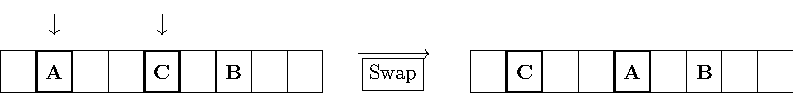
\includegraphics[width=\columnwidth]{figures/swap}
% 		\caption{The \texttt{swap} operator exchanges two randomly selected VMs.}
% 		\label{fig:swap}
% 	\end{subfigure}

% 	\vspace{1.5em}

% 	\begin{subfigure}[T]{\linewidth}
% 		\centering
% 		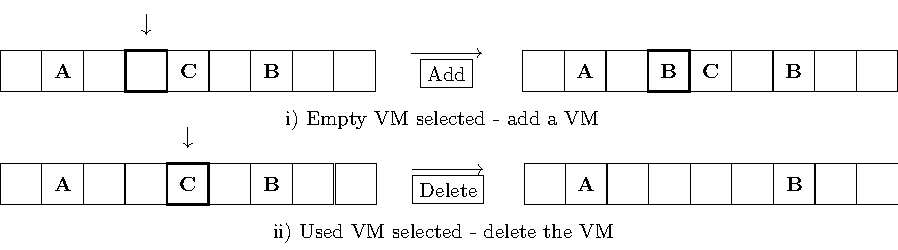
\includegraphics[width=\columnwidth]{figures/add_remove}
% 		\caption{The \texttt{add/delete} operator selects a VM and adds a VM if it is not in use or removes one otherwise.}
% 		\label{fig:add_remove}
% 	\end{subfigure}
% 	\vspace{1em}
% 	\caption{Illustrative examples of the \texttt{swap} and \texttt{add/delete} operators.}
% 	\label{fig:mutation}
% \end{figure}

\subsection{Incorporation into EMO Algorithms}
\label{sec:incorporation}

The solution representation and initialization operators proposed in~\pref{sec:representation} and~\pref{sec:operators} can be incorporated into any EMO algorithm. In this paper, we integrate it into NSGA-II~\cite{DebAPM02} as a proof of concept. It is worth noting that we do not need to make any modification on the environmental selection of the baseline algorithm. \textcolor{red}{Further, we found the classic uniform crossover and mutation reproduction operators to be sufficient to vary and exchange information on the number and position of service instances.}
